%% SECTION HEADER /////////////////////////////////////////////////////////////////////////////////////
\section{GW Propagation in the Real Honeycomb Core Model}
\label{sec:honeycomb}

%% SECTION CONTENT ////////////////////////////////////////////////////////////////////////////////////
All structures used to create the sample were modeled in the simulation with the following elements: 2D for the core, epoxy adhesive and cyanoacrylate glue and 3D for the \ac{cfrp} plate and \acp{pzt}.
During the creation of the mesh, special attention was taken to reduce the number of non-zero values in the matrix \(\textbf{G}\). While the inversion of the matrix \(\left [\textbf{GL}_+^{-1}\textbf{G}^T\right ]\) is necessary to calculate the vector of Lagrange multipliers in \mbox{Equation~(\ref{eq:lambda})} and \(\textbf{L}_+\) is a diagonal matrix, the sparsity of the matrix \(\textbf{G}\) has a significant effect on the computation cost.

One spectral element was intended for each wall of the honeycomb core, while the meshes of the skin plate and the adhesive layer were divided by three rhombus elements per area under the core cell.
In this way, the interface nodes coincide with the nodes lying on the hexagon edges (red line on Figure~\ref{fig:skin_mesh}(\textbf{b})).

The mesh for the cyanoacrylate adhesive consisted of five elements, with a second-order curve at the structure boundary as it is presented in Fig.~\ref{fig:skin_mesh}(\textbf{c}).
This mesh was connected to the the skin with the non-matching interface elements.
The \ac{pzt} mesh coincides with the glue mesh and they are connected with the matching interface elements.
\begin{figure}[H]
	\begin{center}
		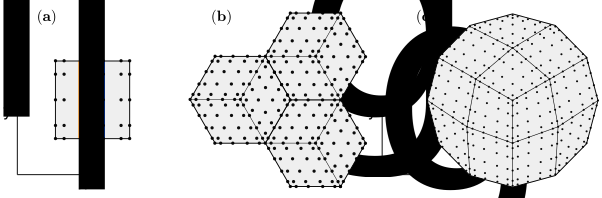
\includegraphics{Chapter_5/skin_mesh}
	\end{center}
	\caption{The mesh with the node distribution, (\textbf{a}) spectral element used for modeling the wall of the core, (\textbf{b}) excerpt of the skin plate and (\textbf{c}) cyanoacrylate glue mesh with the second-order curve at the boundary.}
	\label{fig:skin_mesh}
\end{figure}

The convergence of the solution requires time increment to be less than a critical value, above which the displacements go to infinity.
In the present model, convergence was achieved for \(\Delta t=\)\num{12.2e-3} \(\mu\)s.
The number of nodes for the particular elements are as follows: the core \(6 \times 5\), epoxy adhesive and cyanoacrylate glue \(6 \times 6\), the plate \(6 \times 6 \times 4\) and \acp{pzt} \(6 \times 6 \times 3\).
While the max length of the skin element is six mm, such a \ac{cfrp} model satisfies the condition of at least six nodes per wavelength for the \ac{a0}, as it is the shortest mode propagating in the assumed frequency range.
Table~\ref{tab:wavelength} shows the \ac{a0} wavelengths for various frequency and propagation angles.
\begin{table}[H]
	\small
	\tabcolsep=0.75cm
	%\centering
	\caption{\label{tab:wavelength}The wavelength of the \ac{a0} mode propagated in the presented \ac{cfrp} plate.}
	\begin{tabular}{cccccc}
		\toprule
		\textbf{Frequency} & \multicolumn{5}{c}{\textbf{Propagation angle}}\\
		kHz & \(0^{\circ}\) & \(30^{\circ}\) & \(45^{\circ}\) & \(60^{\circ}\) & \(90^{\circ}\)\\
		\midrule
		50 & 16.5& 15.2&15.0&15.2&16.6\\
		100 & 10.3& 9.6&9.5&9.6&10.3\\
		150 & 7.5& 7.1&7.0&7.1&7.5\\
		\bottomrule
		\multicolumn{6}{r}{{\scriptsize{source: Dispersion Calculator v1.9}}}
	\end{tabular}
\end{table}